\chapter{Berechnung der Tonsysteme}

\begin{enumerate}[a)]
\item

\item
\bfseries{Berechnungsvorschriften}

\begin{align*}
    f(n) &= \sqrt[12]{2} * f_0 & \text{Gleichstufig}
\end{align*} 


\begin{figure}[H]
    \center
    %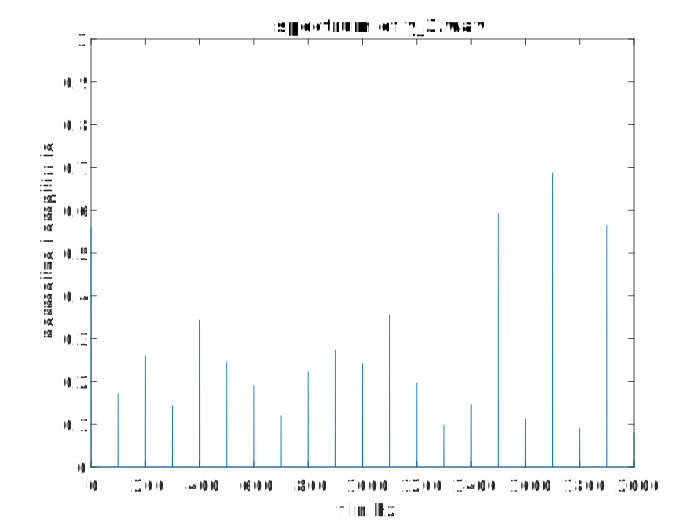
\includegraphics[width = 0.7\textwidth]{Figures/spectrum3.pdf}
    \caption{Betragsspektrum von y\_3.wav}
    \label{fig:bs3}
\end{figure}


\end{enumerate}